
%(BEGIN_QUESTION)
% Copyright 2006, Tony R. Kuphaldt, released under the Creative Commons Attribution License (v 1.0)
% This means you may do almost anything with this work of mine, so long as you give me proper credit

{\it Stilling wells} are very useful accessories to many types of liquid level measurement gauges, including float and ultrasonic.  However, if used on a liquid-liquid interface level measurement application, care must be taken to ensure the stilling well is always submerged:

$$\includegraphics[width=15.5cm]{i00315x01.eps}$$

Explain why a stilling well might be used in a liquid level measurement system, and also why it needs to be completely submerged if being used to measure the level of an interface.

\underbar{file i00315}
%(END_QUESTION)





%(BEGIN_ANSWER)

If not completely submerged, the interface level in the well might not match the interface level in the rest of the vessel.

%(END_ANSWER)





%(BEGIN_NOTES)

Examples of what could happen if the pipe were not fully submerged:

$$\includegraphics[width=15.5cm]{i00315x02.eps}$$

Without liquid access through the top of the stilling well, the height of the light liquid column in the pipe can never change!

%INDEX% Measurement, interface level: use of stilling well

%(END_NOTES)


